%% %%%%%%%%%%%%%%%%%%%%%%%%%%%%%%%%%%%%%%%%%%%%%%%%%
%% Template for a conference paper, prepared for the
%% Food and Resource Economics Department - IFAS
%% UNIVERSITY OF FLORIDA
%% %%%%%%%%%%%%%%%%%%%%%%%%%%%%%%%%%%%%%%%%%%%%%%%%%
%% Version 1.0 // November 2019
%% %%%%%%%%%%%%%%%%%%%%%%%%%%%%%%%%%%%%%%%%%%%%%%%%%
%% Ariel Soto-Caro
%%  - asotocaro@ufl.edu
%%  - arielsotocaro@gmail.com
%% %%%%%%%%%%%%%%%%%%%%%%%%%%%%%%%%%%%%%%%%%%%%%%%%%
\documentclass[11pt]{article}
\usepackage{UF_FRED_paper_style}

\usepackage{lipsum}  %% Package to create dummy text (comment or erase before start)

%% ===============================================
%% Setting the line spacing (3 options: only pick one)
% \doublespacing
% \singlespacing
\onehalfspacing
%% ===============================================

\setlength{\droptitle}{-5em} %% Don't touch

% %%%%%%%%%%%%%%%%%%%%%%%%%%%%%%%%%%%%%%%%%%%%%%%%%%%%%%%%%%
% SET THE TITLE
% %%%%%%%%%%%%%%%%%%%%%%%%%%%%%%%%%%%%%%%%%%%%%%%%%%%%%%%%%%

% TITLE:
\title{nacimiento de la computación}

% AUTHORS:
\author{Jhon Ricardo Rios\\% Name author
    \href{mailto:jhon.rios1@udea.edu.co}{\texttt{jhon.rios1@udea.edu.co}} %% Email author 1 
    }
% DATE:
\date{\today}

% %%%%%%%%%%%%%%%%%%%%%%%%%%%%%%%%%%%%%%%%%%%%%%%%%%%%%%%%%%
% %%%%%%%%%%%%%%%%%%%%%%%%%%%%%%%%%%%%%%%%%%%%%%%%%%%%%%%%%%
\begin{document}
% %%%%%%%%%%%%%%%%%%%%%%%%%%%%%%%%%%%%%%%%%%%%%%%%%%%%%%%%%%
% %%%%%%%%%%%%%%%%%%%%%%%%%%%%%%%%%%%%%%%%%%%%%%%%%%%%%%%%%%
% ABSTRACT
% %%%%%%%%%%%%%%%%%%%%%%%%%%%%%%%%%%%%%%%%%%%%%%%%%%%%%%%%%%
% %%%%%%%%%%%%%%%%%%%%%%%%%%%%%%%%%%%%%%%%%%%%%%%%%%%%%%%%%%
{\setstretch{.8}
\maketitle
% %%%%%%%%%%%%%%%%%%

}

% %%%%%%%%%%%%%%%%%%%%%%%%%%%%%%%%%%%%%%%%%%%%%%%%%%%%%%%%%%
% %%%%%%%%%%%%%%%%%%%%%%%%%%%%%%%%%%%%%%%%%%%%%%%%%%%%%%%%%%
% BODY OF THE DOCUMENT
% %%%%%%%%%%%%%%%%%%%%%%%%%%%%%%%%%%%%%%%%%%%%%%%%%%%%%%%%%%
% %%%%%%%%%%%%%%%%%%%%%%%%%%%%%%%%%%%%%%%%%%%%%%%%%%%%%%%%%%

% --------------------
\section{Introduction}
% --------------------

\begin{center}
Desde que se crearon las matemáticas han sido útiles para el vivir diario y siempre han habido
personajes que han hecho grandes aportes a este campo tales como Pitágoras, Isaac Newton, Alan Turing, por mencionar algunos,
con las matemáticas se han logrado resolver muchos problemas pero habían algunos que no eran posibles de resolver ya que las matemáticas no eran consistentes y se evidencio que los fundamentos en los cuales está se basa no estaban bien definidos, a esto se le conoce como la crisis de los fundamentos, en este texto veremos en que consiste la crisis, que desencadeno este hecho para la computación y quienes fueron los encargados de solucionar dicho problema.
\end{center}

% --------------------
\section{Desarrollo}
\cite{ferreiros2004episodio}
% --------------------

\begin{center}
    
\end{center}
\citep{Chavas2015} % Example of citation. Erase before use

% --------------------
\section{Conclusiones}
% --------------------

\begin{center}
    
\end{center}


% %%%%%%%%%%%%%%%%%%%%%%%%%%%%%%%%%%%%%%%%%%%%%%%%%%%%%%%%%%
% %%%%%%%%%%%%%%%%%%%%%%%%%%%%%%%%%%%%%%%%%%%%%%%%%%%%%%%%%%
% REFERENCES SECTION
% %%%%%%%%%%%%%%%%%%%%%%%%%%%%%%%%%%%%%%%%%%%%%%%%%%%%%%%%%%
% %%%%%%%%%%%%%%%%%%%%%%%%%%%%%%%%%%%%%%%%%%%%%%%%%%%%%%%%%%
\medskip

\bibliography{references.bib} 

\newpage

% %%%%%%%%%%%%%%%%%%%%%%%%%%%%%%%%%%%%%%%%%%%%%%%%%%%%%%%%%%
% FIGURES
% %%%%%%%%%%%%%%%%%%%%%%%%%%%%%%%%%%%%%%%%%%%%%%%%%%%%%%%%%%
% %%%%%%%%%%%%%%%%%%%%%%%%%%%%%%%%%%%%%%%%%%%%%%%%%%%%%%%%%%

\begin{figure}[H]
    \centering
        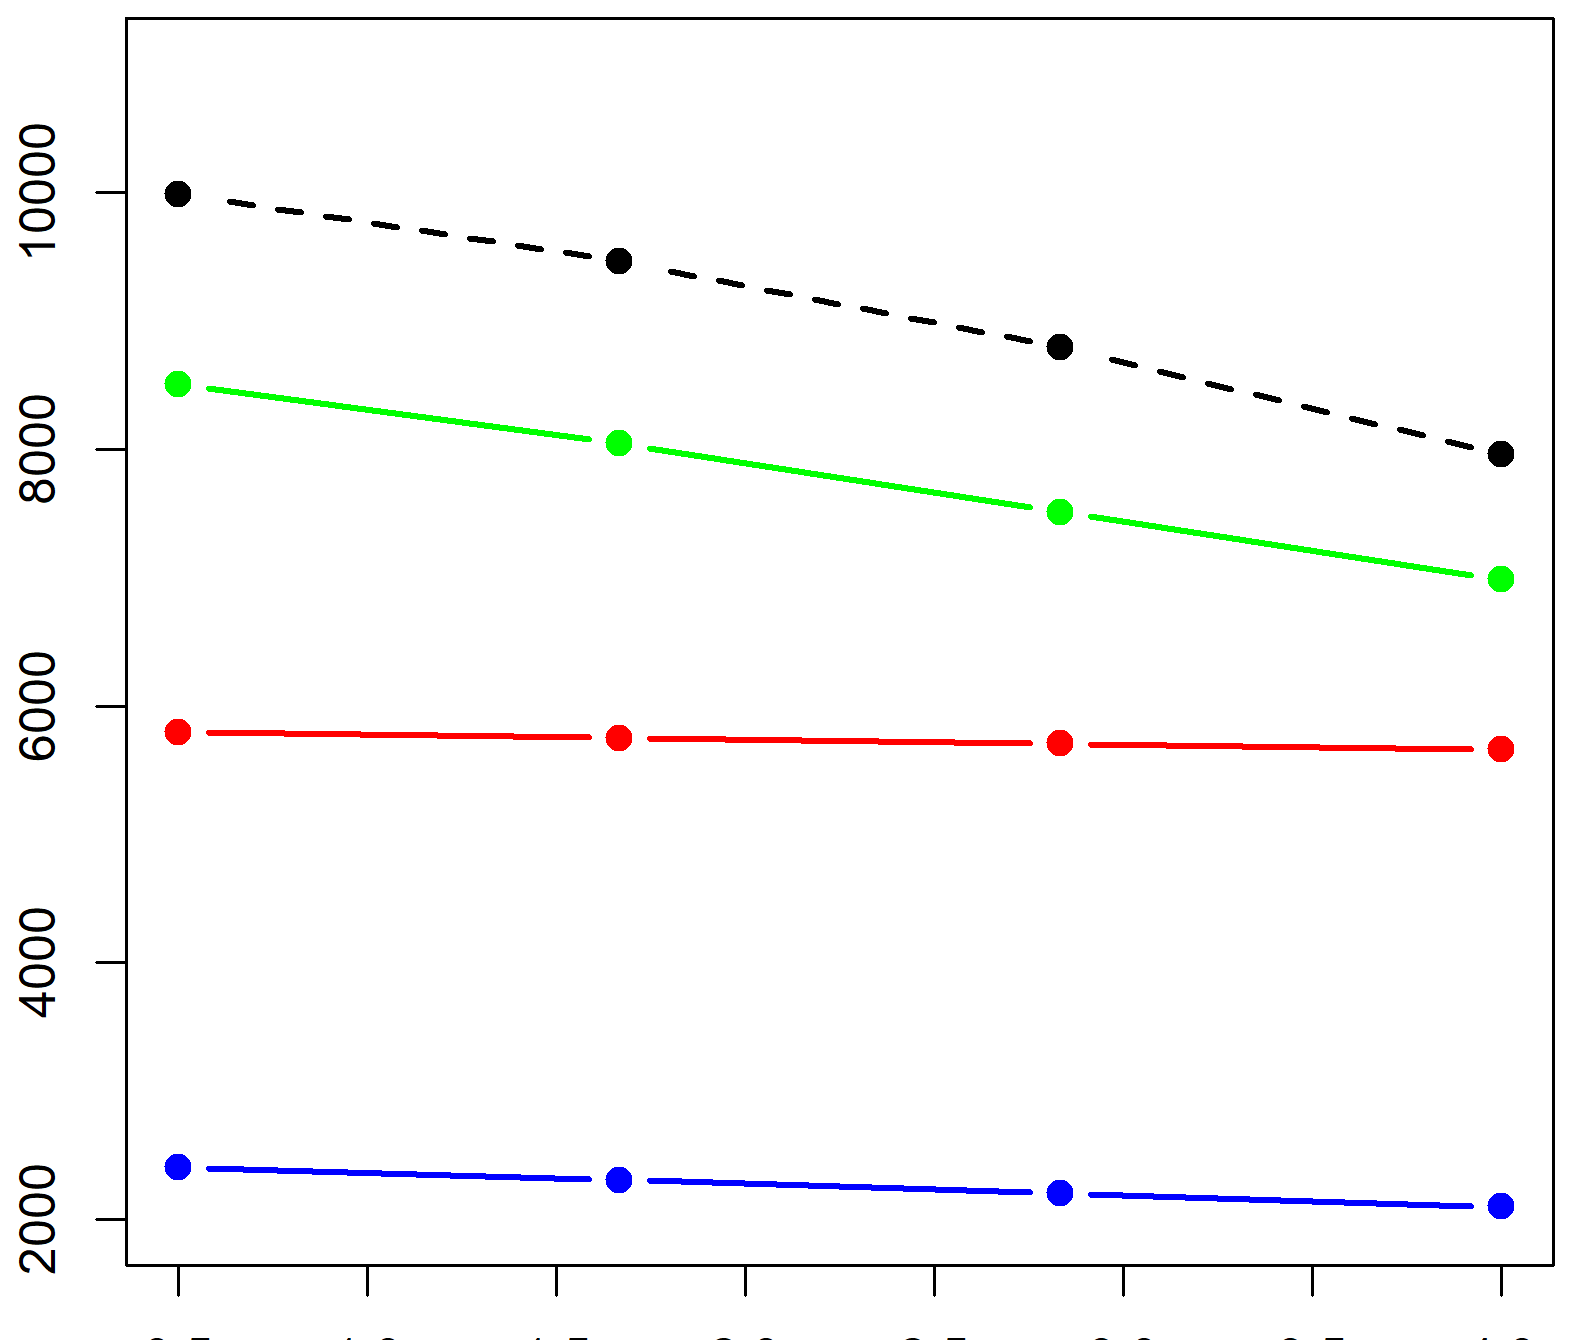
\includegraphics[scale=.8]{figures/example_figure.png}
    \caption{Example figure.}
    \label{fig:1}
\end{figure}

% ==========================
% ==========================
% ==========================


\end{document}